\documentclass[aspectratio=169,11pt]{beamer}
\usepackage[T1]{fontenc}
\usepackage{lmodern,booktabs,amsmath}
\usepackage{tikz}
\usetikzlibrary{arrows.meta,positioning,fit,calc}
\definecolor{Ink}{HTML}{17324D}
\definecolor{Accent}{HTML}{147D72}
\definecolor{Soft}{HTML}{E8F2F1}
\definecolor{NavyBlue}{HTML}{17324D}
\definecolor{ForestGreen}{HTML}{147D72}
\setbeamercolor{normal text}{fg=Ink,bg=white}
\setbeamercolor{frametitle}{fg=Ink,bg=white}
\setbeamercolor{structure}{fg=Accent}
\setbeamercolor{block title}{fg=white,bg=Ink}
\setbeamercolor{block body}{fg=Ink,bg=Soft}
\setbeamertemplate{navigation symbols}{}
\setbeamertemplate{footline}{\hfill\scriptsize Authorized Agent Workflows\hspace{1em}\insertframenumber/10\hspace{1.4em}\vspace{0.65em}}
\setbeamertemplate{itemize item}{\color{Accent}$\blacktriangleright$}
\setbeamertemplate{itemize subitem}{\color{Accent}$\bullet$}
\setlength{\leftmargini}{1.5em}
\title{Authorized Agent Workflows}
\subtitle{A research agenda for valuable, permitted work}
\author{newdarwindev}
\date{October 2026}
\begin{document}

\begin{frame}[plain]
\vspace{0.6cm}
{\color{Accent}\Large POSITION PAPER}\par\vspace{0.7cm}
{\Huge\bfseries Authorized Agent\\Workflows}\par\vspace{0.35cm}
{\Large A research agenda for valuable, permitted work}\par\vfill
{\small newdarwindev \quad | \quad October 2026}\par\vspace{0.5cm}
\end{frame}

\begin{frame}{A strong thesis, stated as a hypothesis}
\begin{block}{Commercial proposition}
For some teams outside frontier labs, the largest near-term research opportunity may be turning general models into systems that complete valuable, owner-authorized tasks across real accounts and services.
\end{block}
\vspace{0.25cm}
\begin{itemize}
\item The model may know the next step while the product lacks a permitted execution path.
\item Research target: verified task outcomes, including handoff and recovery.
\item ``Greatest'' requires comparison with stronger models, ordinary software, and vertical products.
\end{itemize}
\vfill
{\tiny Motivation: Zhou et al., WebArena (2023); Drouin et al., WorkArena (2024). Historical benchmarks are not current market estimates.}
\end{frame}

\begin{frame}{First diagnose why a task stopped}
\small
\begin{tabular}{p{0.24\linewidth}p{0.66\linewidth}}
\toprule
Cause & Appropriate response\\\midrule
Capability & Improve perception, reasoning, or planning.\\
Integration & Add a reliable API, tool, browser adapter, or durable state.\\
Authorization & Ask the owner or administrator for a specific grant.\\
Policy refusal & Record a product or safety denial; preserve the boundary.\\
Platform restriction & Use an allowed route or human operation; stop if neither exists.\\\bottomrule
\end{tabular}
\vfill
\begin{block}{Scoring rule}
A filled form, draft, or click is progress. Completion requires the requested remote state, permission, and evidence.
\end{block}
\end{frame}

\begin{frame}{Model the goal, authority, and remote state}
\large
\[T=(g,E,A,P,B)\]
\normalsize
Goal $g$; environment $E$; authority record $A$; policy $P$; budget $B$.
\vspace{0.35cm}
\begin{columns}[T]
\begin{column}{0.48\linewidth}
\begin{block}{Executable action}
Technically available \emph{and} permitted for this principal, resource, scope, purpose, and time.
\end{block}
\end{column}
\begin{column}{0.48\linewidth}
\begin{block}{Successful task}
Goal reached \emph{and} action path authorized \emph{and} outcome independently verified.
\end{block}
\end{column}
\end{columns}
\vspace{0.3cm}
An external timeout can leave the outcome \textbf{unknown}. Reconcile before retrying a write.
\end{frame}

\begin{frame}{Proposed system boundary}
\centering
\resizebox{0.92\linewidth}{!}{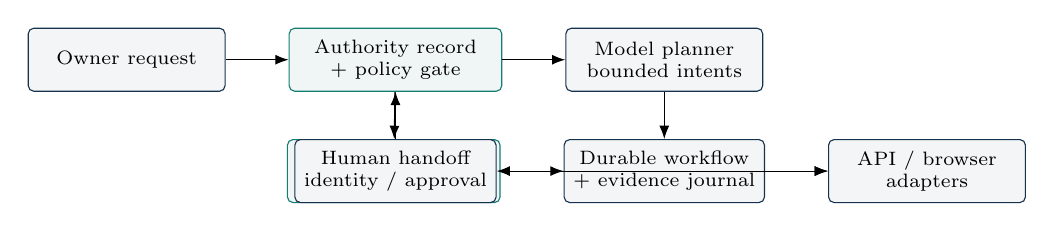
\begin{tikzpicture}[>=Latex, node distance=6mm and 8mm, every node/.style={font=\scriptsize},
  box/.style={draw=NavyBlue,rounded corners=2pt,fill=NavyBlue!5,align=center,minimum height=8mm,minimum width=25mm},
  gate/.style={draw=ForestGreen,rounded corners=2pt,fill=ForestGreen!7,align=center,minimum height=8mm,minimum width=27mm}]
\node[box] (owner) {Owner request};
\node[gate,right=of owner] (auth) {Authority record\\+ policy gate};
\node[box,right=of auth] (planner) {Model planner\\bounded intents};
\node[box,below=of planner] (flow) {Durable workflow\\+ evidence journal};
\node[gate,left=of flow] (broker) {Credential broker\\scoped retrieval};
\node[box,right=of flow] (adapter) {API / browser\\adapters};
\node[box,below=of auth] (human) {Human handoff\\identity / approval};
\draw[->] (owner) -- (auth);
\draw[->] (auth) -- (planner);
\draw[->] (planner) -- (flow);
\draw[->] (flow) -- (adapter);
\draw[->] (broker) -- (adapter);
\draw[->] (auth) -- (broker);
\draw[<->] (flow) -- (human);
\draw[->] (human) -- (auth);
\end{tikzpicture}
}
\vspace{0.45cm}
\begin{itemize}
\item Planner sees bounded capabilities; policy and credentials live outside its context.
\item Durable workflow records intent, approval, effect evidence, and uncertainty.
\item Public components such as OpenBao and Temporal are illustrative, not a measured deployment.
\end{itemize}
\end{frame}

\begin{frame}{Credentials: custody is part of the research}
\begin{columns}[T]
\begin{column}{0.5\linewidth}
\textbf{Minimum viable boundary}
\begin{itemize}
\item Owner grants a scoped API token or approved session.
\item Broker binds retrieval to task, principal, tool, and destination.
\item Adapter uses the credential; model and logs never receive its value.
\end{itemize}
\end{column}
\begin{column}{0.46\linewidth}
\begin{block}{Two distinctions}
Vault storage does not make a website password dynamically revocable. Browser authentication state can impersonate its owner.
\end{block}
\end{column}
\end{columns}
\vfill
{\tiny Sources: OpenBao lease/database documentation; Playwright authentication documentation.}
\end{frame}

\begin{frame}{Enrollment and publishing need explicit handoff}
\small
\begin{columns}[T]
\begin{column}{0.49\linewidth}
\textbf{Account enrollment}
\begin{enumerate}
\item Prepare owner-supplied fields.
\item Pause for identity checks and binding acceptance.
\item Verify the resulting account state.
\end{enumerate}
\end{column}
\begin{column}{0.49\linewidth}
\textbf{Social publication}
\begin{enumerate}
\item Identify account, audience, content, and approved route.
\item Obtain specific content approval.
\item Publish through a permitted API or hand off; verify the object.
\end{enumerate}
\end{column}
\end{columns}
\vspace{0.5cm}
\begin{block}{Separate gates}
Account authority, content approval, and platform permission are different facts. An OAuth token alone does not settle the last one.
\end{block}
\end{frame}

\begin{frame}{Durability cannot promise exactly-once effects}
\begin{itemize}
\item A worker may retry after an external write succeeded but its completion report was lost.
\item Reads are often safe to retry; public writes require effect reconciliation.
\item Keep \textbf{unknown} as a real task state when the remote effect cannot be established.
\end{itemize}
\vspace{0.25cm}
\begin{block}{Example: publish timeout}
Query the remote object or ask the owner to reconcile before another submission. A blind retry can make a duplicate.
\end{block}
\vfill
{\tiny Source: Temporal Activity Definition documentation.}
\end{frame}

\begin{frame}{Evaluate the authorized outcome, not the demo}
\small
\begin{columns}[T]
\begin{column}{0.5\linewidth}
\textbf{Matched baselines}
\begin{itemize}
\item Human-only process
\item Deterministic integration
\item Tool-only agent
\item Same model + authority-aware workflow
\end{itemize}
\end{column}
\begin{column}{0.48\linewidth}
\textbf{Report}
\begin{itemize}
\item Verified authorized completion
\item Human active minutes and elapsed time
\item Duplicate effects, policy violations, unknowns
\item Total cost per successful task
\end{itemize}
\end{column}
\end{columns}
\vspace{0.35cm}
Use repeated trials and hold out sites, account configurations, and task templates. Correct denial is a valid outcome for a disallowed request.
\vfill
{\tiny Methods: $\tau$-bench (2024); Kapoor et al., AI Agents That Matter (2024).}
\end{frame}

\begin{frame}{The agenda is falsifiable}
\small
\begin{enumerate}
\item Test whether orchestration improves verified completion with the model fixed.
\item Measure whether external custody lowers exposure without excessive owner effort.
\item Test whether handoff states reduce duplicates and false completion claims.
\item Compare with stronger models and conventional software on value per engineering dollar.
\end{enumerate}
\vspace{0.3cm}
\begin{block}{Open result}
Frontier providers may solve the gap; deterministic software may win; secret custody may cost too much. The ``greatest opportunity'' claim survives only where matched evidence supports it.
\end{block}
\end{frame}
\end{document}
